过渡态理论(TST)有助于解释基元反应的速率。过渡态理论中假定反应物和过渡态之间存在准平衡过程。

\begin{figure}[h]
	\centering
	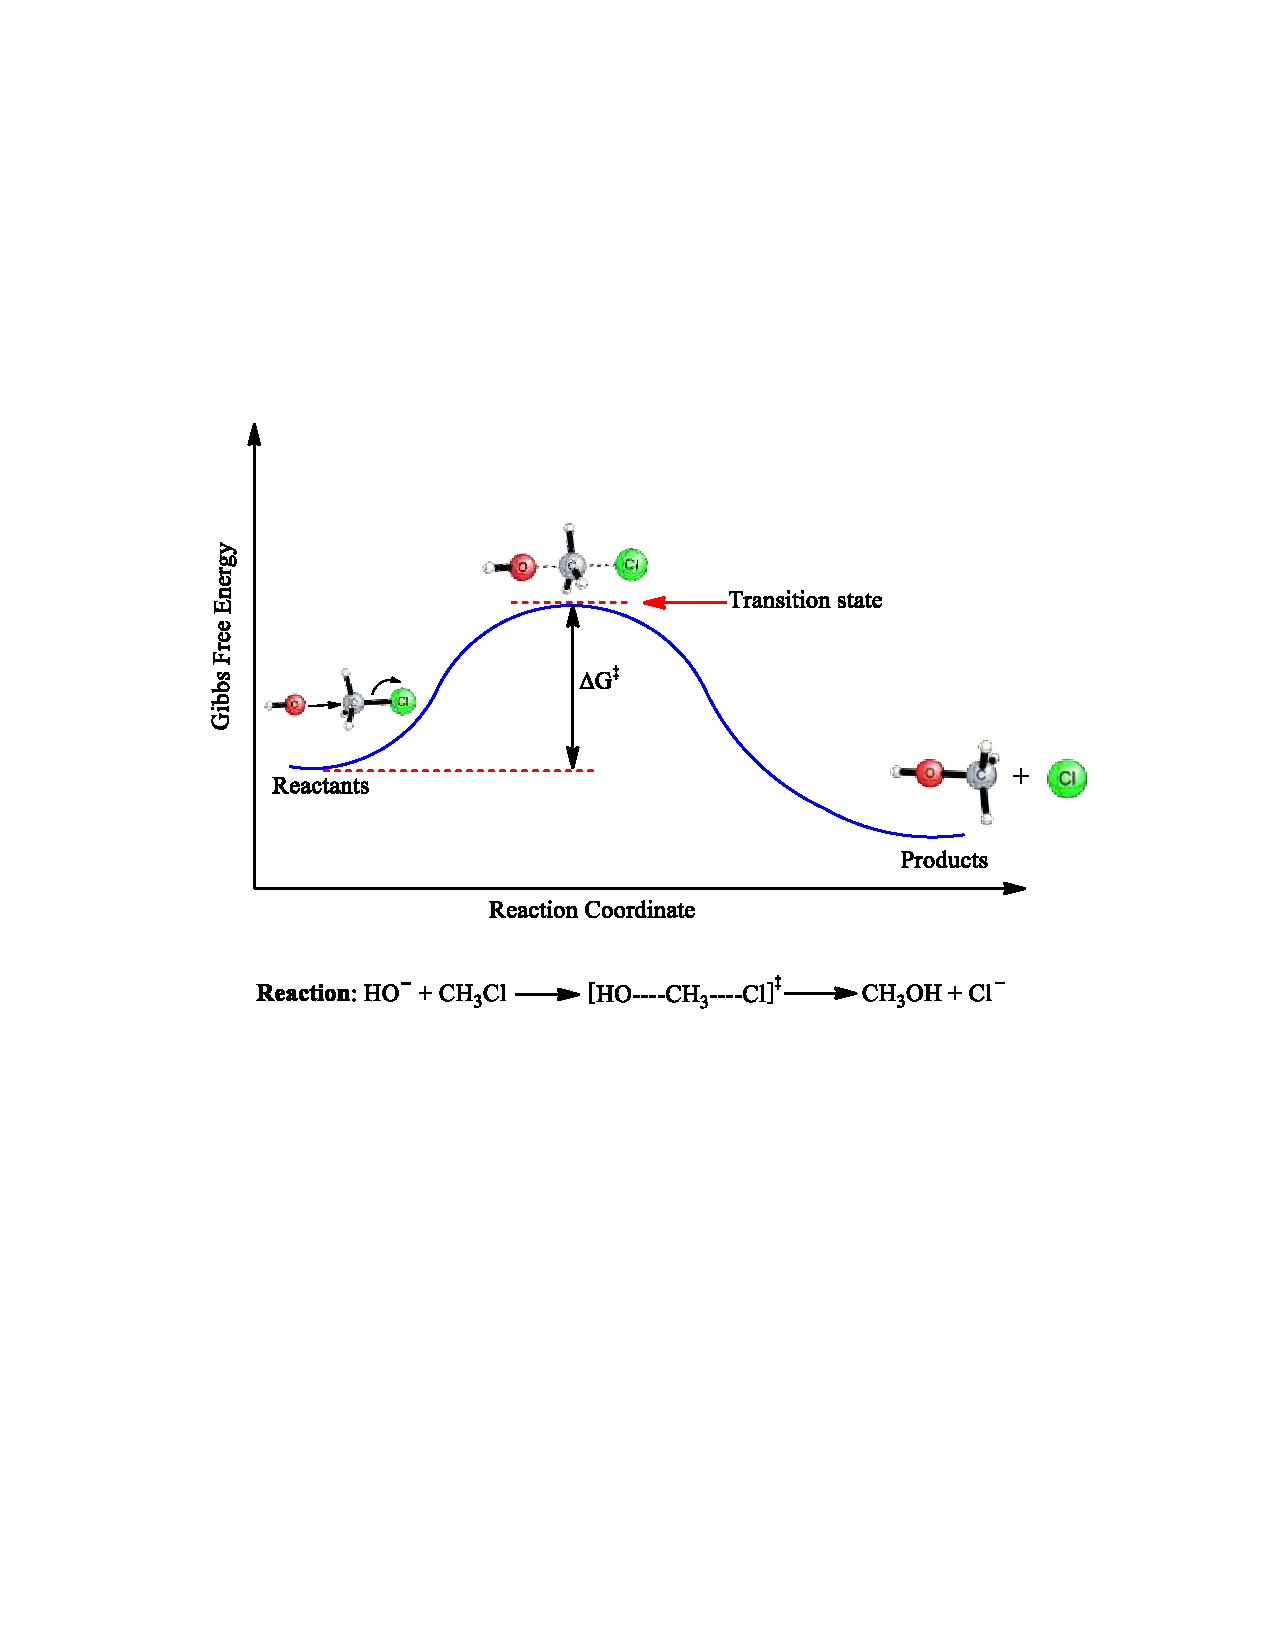
\includegraphics[width=15cm]{./pic/t21-1.pdf}
\end{figure}

与阿伦尼乌斯模型类似,过渡态理论中速率常数和温度的关系如下所示:

$$K_{\mathrm{TST}} = \frac{k_BT}{h} \exp\left[- \frac{\Delta G^{\neq}}{RT}\right]$$

其中,\(k_B\)是玻尔兹曼常数,\(h\)是普朗克常数,\(\Delta G^{\neq}\)是活化自由能。

过渡态理论的速率常数中引入了一个温度相关的项用来替代阿伦尼乌斯因子A。此外,过渡态理论使我们更好的理解了活化能的概念,并架起了理论与实验之间的桥梁。值得注意的是,相比于阿伦尼乌斯模型中常数\(E_a\),过渡态理论中的活化自由能项是温度相关的。

有机化合物的分解反应符合一级反应动力学,其在给定温度下的速率常数如下所示:

\begin{longtable}[]{@{}lllll@{}}
	\toprule
	$t$ (°C) & 10 & 30 & 50 & 70\tabularnewline
	\midrule
	\endhead
	$l$/10\textsuperscript{-4} (s\textsuperscript{-1}) &
	1.1408 & 17.2075 & 185.5042 & 1515.7157\tabularnewline
	\bottomrule
\end{longtable}

\noindent\textbf{21.1.} 根据阿伦尼乌斯模型,计算反应活化能。

\noindent\textbf{21.2.} 计算阿伦尼乌斯因子A。

\noindent\textbf{21.3.} 计算该有机化合物在75 °C下的半衰期。

\noindent\textbf{21.4.}
假设该反应的速率常数满足过渡态理论而不是阿伦尼乌斯模型,试计算30
°C下的活化自由能。

\noindent\textbf{21.5.}
假设从阿伦尼乌斯模型和过渡态理论得到的速率常数相等,试推导出活化焓、活化熵与活化能以及阿伦尼乌斯因子之间的关系。

\noindent\textbf{21.6.} 根据上面得到的表达式,计算在80 °C下的活化焓。

当反应物中一个原子被替换成其同位素后,该反应速率的变化称为动力学同位素效应(KIE)。有机化学中通常使用称为``氘代标记''的方法测定KIE,该方法将分子中一个或多个氢原子替换为氘原子。

动力学同位素效应的一个原因是一级动力学同位素效应。在一级KIE中,反应速率的变化由量子化学因素引起,因为重的同位素的零点振动能(ZPVE)比轻的同位素更低。在过渡态理论之下,氘代后的活化自由能的改变只受到零点振动能的影响。据此,我们可以写出如下公式:

$$\frac{k_H}{k_D} = \frac{\exp[(ZPVE(R, H)-ZPVE(TS,H))/RT]}{\exp[(ZPVE(R, D)-ZPVE(TS, D))/RT]}$$

其中,\(k_H\)和\(k_D\)是含有氢和氘底物各自的速率常数,$ZPVE(R,
H)$和$ZPVE(R,D)$是各自的零点振动能,$ZPVE(TS, H)$和$ZPVE(TS,
D)$是各自过渡态的零点振动能。

对于某有机化合物的分解反应,其氘代底物的过渡态(TS-D)和氢代底物过渡态(TS-H)的零点振动能差为--2.3
kJ/mol,氢代底物(R-H)的零点振动能比氘代底物(R-D)高3.0 kJ/mol。

\noindent\textbf{21.7.} 计算298.15 K下\(\frac{k_H}{k_D}\)的数值。

\noindent\textbf{21.8.} 计算330.0 K下\(\frac{k_H}{k_D}\)的数值。

\noindent\textbf{21.9.} 当\(k_H\)为2.5 × 10\textsuperscript{2},\(k_D\)为2.2 ×
10\textsuperscript{2}时,温度为多少。
